\chapter{Implementation}
\label{c:implementation}

In the thesis, we verify our design by executing \textit{Fountain} on \RRS and selecting \textit{egl} as a remote engine. We present the implementation details in this chapter, and describe how we solve issues in the last four section.

\section{Command Encoding}
\label{s:rsListeningThread}
The following figure shows the encoding of command whose command structure is RS\_CMD\_ScriptInvokeV. The command calls a function declared in \Core{}. In Fountain, the function is adding particulars on the screen and is called everytime the screen touched. 

The first field of the command is CMD\_ID, which is a integer(i.e., \textit{uint32\_t}, 4 bytes) representing a CMD type. The CMD\_ID table is defined in \textit{rsgApiStructs.h}. The second field is the size used in the command. To get the size, we should know what fields are in the structure of RS\_CMD\_ScriptInvokeV. According to the figure \ref{fig:ScriptInvokeCMDEncoding}, we could know that there are four fields in the structure. RsScript is a pointer to \textit{Script} object.(mentioned in \ref{s:RSObject}), slot means the slot number for reflection, and the last two fields stores the informantion of the funciton arguments which including the size and data. In \Fountain{}, it inlcudes X-coordinate, Y-coordinate, the pressure andt etc. 

Back to the encoding, the third field means the size of argument data. And we use the fourth field for distinguish if the command needs a synchronization, i.e., distinguish between \textit{send()} and \textit{sendSync()}. The last two fields handle the information of the structure. 

\begin{center-figure}
	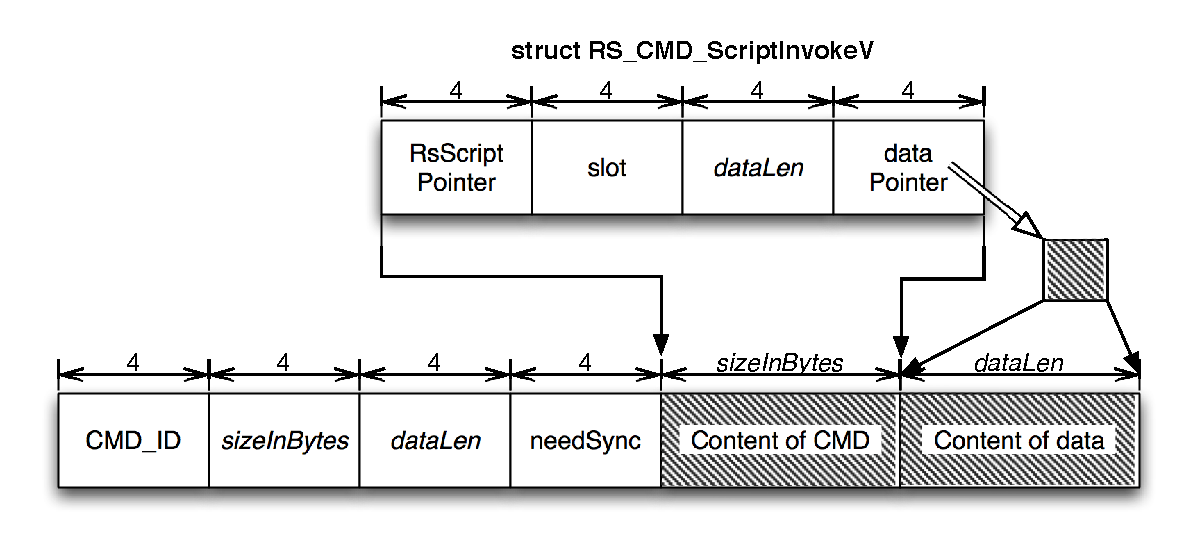
\includegraphics[scale=0.8]{fig/ScriptInvokeCMDEncoding.eps}
	\caption{RS\_CMD\_ScriptInvokeV encoding}
	\label{fig:ScriptInvokeCMDEncoding}
\end{center-figure}

\section{Transport Layer}
\label{s:rsListeningThread}
To receive commands, we choose socket to build \Transport{} for the the following reasons: (1) We need a lower-level implementation in \Core{}; (2) Bi-directional communication; and (3) Better performance of server side.

After the creation of RS context thread, we dynamically create the RS listening thread that depends on Android property. The following code shows our implementation.

\begin{lstlisting}
if (props.mRemoteServer) {
    pthread_t listeningThreadID;
    LOGV("create rsListeningThread");
    status = mIO.mToCore.receive(&listeningThreadID, &threadAttr, this);
    if (status) {
        LOGE("Failed to start rsListeningThread.");
        return false;
    }    
} else if (props.mRemoteClient){
    mIO.mToCore.initSocket();
} 
\end{lstlisting}

\paragraph{Server or Client?} The library of \RRS{} should support not only the client but also the server. A library for server and the other for client doesn't make sense if we want to accomplish the feature of two-way communication. For the reason, we stores the information through Android property system. For example, \RRS{} gets the property from \verb|props.mRemoteServer| and creates the RS listening thread if you type this in the ADB: 
\\\\ \verb|adb shell setprop remote.rs.server 1|\\\\

The idea of \RRS{} is straightforward, but it's still some issues we should take care. The following four subsection describes the challenge we encounter when extending \RS{} to \RRS{}.

\section{Replicated Command}
\label{s:rsListeningThread}
The key idea of \RRS{} is replaying the commands on the remote engine. Initially, any kind of \textit{commit()} and \textit{commitSync()} commands are followed by \textit{send()} and \textit{sendSync()} respectively.\footnote{Actually, we use sendCMD() instead of send() to avoid the confusion with socket send().} As a result, we found that it caused a error due to those replicated executed commands. For instance, binding the fragment twice might lead to chaos. The commands used for initialization should not be executed on the individual engine. In \Fountain{}, they are listed below in order:\\
\verb|RS_CMD_ID_ContextSetSurface|\\
\verb|RS_CMD_ID_ProgramFragmentCreate|\\
\verb|RS_CMD_ID_ContextBindProgramFragment|\\
\verb|RS_CMD_ID_ElementCreate|\\
\verb|RS_CMD_ID_ElementCreate2|\\
\verb|RS_CMD_ID_MeshCreate|\\
\verb|RS_CMD_ID_MeshBindIndex|\\
\verb|RS_CMD_ID_MeshBindVertex|\\
\verb|RS_CMD_ID_MeshInitVertexAttribs|\\
\verb|RS_CMD_ID_ScriptCCreate|\\
\verb|RS_CMD_ID_ScriptSetVarObj|\\
\verb|RS_CMD_ID_ScriptBindAllocation|\\
\verb|RS_CMD_ID_ContextBindRootScript|\\

\section{Command Synchornization}
\label{s:rsListeningThread}

As we mentioned in in prior chapter, a part of commands are put into the command queue via \textit{commitSync()}. That means \Client{} should be blocked until the command is flushed in \Core{}. Flushing in \RS{} refers to no command in the command queue. We demonstrate the design in Figure \ref{fig:LocklessFifo_pointer}. There are three markers in the figure:
\begin{itemize}
\item\textit{mGet} points to the memory address where the next command will be put.
\item\textit{mPut} points to the memory address where the next command will be popped.
\item\textit{mEnd} points to the memory address of end of the queue.
\end{itemize}
\begin{center-figure}
	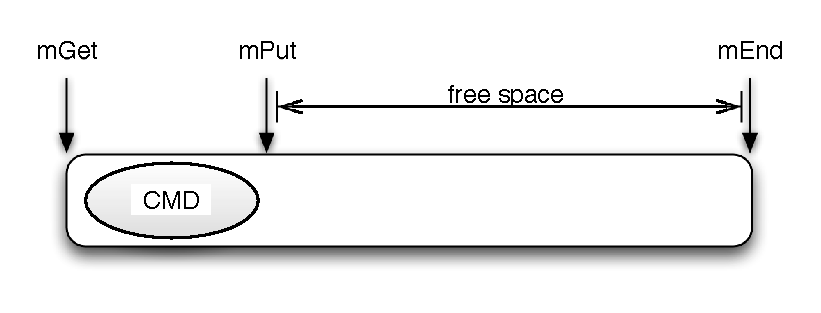
\includegraphics[scale=0.8]{fig/LocklessFifo_pointer.eps}
	\caption{Lockless FIFO command queue}
	\label{fig:LocklessFifo_pointer}
\end{center-figure}

Therefore, the command queue is flushed \textbf{if \textit{mGet} is equal to \textit{mPut}}.

Note that we have a \textit{sendSync()} for \RRS{}, the difference is the client (which sends the command) should be blocked instead of the server.

\section{Allocation of Command Queue}
\label{s:rsListeningThread}
Another stuff we should take care of the command queue is the allocation. In \RS{} implementation, either \textit{mToCore} or \textit{mToClient} are represented as a pointer and passed through functions by pointer. If we still pass the pointer to remote engine, it might cause a segamentation fault. As a result, we should remove it and get the correct \textit{mToCore} pointer.

\section{Handle the Pointer}
\label{s:rsListeningThread}
Like the allocation of command queue, almost variable are refered by pointer. So we should take care of it. For example, in \Fountain{}, we did that as the below:
\begin{lstlisting}
static inline void rsHCAPI_ScriptInvokeV (RsContext rsc, RsScript va, uint32_t slot, const void * data, uint32_t sizeBytes) {
    ThreadIO *io = &((Context *)rsc)->mIO;
    uint32_t size = sizeof(RS_CMD_ScriptInvokeV);
    if (sizeBytes < DATA_SYNC_SIZE) {
        size += (sizeBytes + 3) & ~3; 
    }   
    RS_CMD_ScriptInvokeV *cmd = static_cast<RS_CMD_ScriptInvokeV *>(io->mToCore.reserve(size));
    cmd->s = va; 
    cmd->slot = slot;
    cmd->dataLen = sizeBytes;
    cmd->data = data; 
    if (sizeBytes < DATA_SYNC_SIZE) {
        cmd->data = (void *)(cmd+1);
        memcpy(cmd+1, data, sizeBytes);
        io->mToCore.commit(RS_CMD_ID_ScriptInvokeV, size);
        if (&((Context *)rsc)->props.mRemoteClient)
            io->mToCore.sendCMD(RS_CMD_ID_ScriptInvokeV, size, cmd, cmd->dataLen, 0); 
    } else {
        io->mToCore.commitSync(RS_CMD_ID_ScriptInvokeV, size);
        io->mToCore.sendSync(RS_CMD_ID_ScriptInvokeV, size);
    }   

}
\end{lstlisting}


%1. 命令是會重複的, 不是所有的命令都需要傳送(有些是初始化動作)
%2. 有兩種命令,我們必須處理同步問題
%3. command queue 記憶體位址
%4. 有些命令的參數是包含指標的!





